\documentclass[12pt]{article}
\usepackage{graphicx}
%\documentclass[journal,12pt,twocolumn]{IEEEtran}
\usepackage[none]{hyphenat}
\usepackage{graphicx}
\usepackage{listings}
\usepackage[english]{babel}
\usepackage{graphicx}
\usepackage{caption}
\usepackage{hyperref}
\usepackage{booktabs}
\usepackage{array}
\usepackage{amsmath}   % for having text in math mode
\usepackage{listings}
\lstset{
  frame=single,
  breaklines=true
}
%New macro definitions
\newcommand{\mydet}[1]{\ensuremath{\begin{vmatrix}#1\end{vmatrix}}}
\providecommand{\brak}[1]{\ensuremath{\left(#1\right)}}
\providecommand{\norm}[1]{\left\lVert#1\right\rVert}
\newcommand{\solution}{\noindent \textbf{Solution: }}
\newcommand{\myvec}[1]{\ensuremath{\begin{pmatrix}#1\end{pmatrix}}}
\let\vec\mathbf

\begin{document}
\begin{center}
\textbf\large{CHAPTER-7 \\ COORDINATE GEOMETRY}
\end{center}

\section*{EXERCISE - 7.2}
\begin{enumerate}

\item Find the coordinates of the point which divides the join of $(-1,7) \text{ and } (4,-3)$ in the ratio 2:3.
\item Find the coordinates of the points of trisection of the line segment joining $(4,-1) \text{ and } (-2,3)$.

\item To conduct Sports Day activities, in your rectangular shaped school                   
ground ABCD, lines have 
drawn with chalk powder at a                 
distance of 1m each. 100 flower pots have been placed at a distance of 1m 
from each other along AD, as shown 
in Fig. 7.12. Niharika runs $ \frac {1}{4} $th the 
distance AD on the 2nd line and 
posts a green flag. Preet runs $ \frac {1}{5} $th 
the distance AD on the eighth line 
and posts a red flag. What is the 
distance between both the flags? If 
Rashmi has to post a blue flag exactly 
halfway between the line segment 
joining the two flags, where should 
she post her flag?
\begin{figure}[h!]
  \centering
  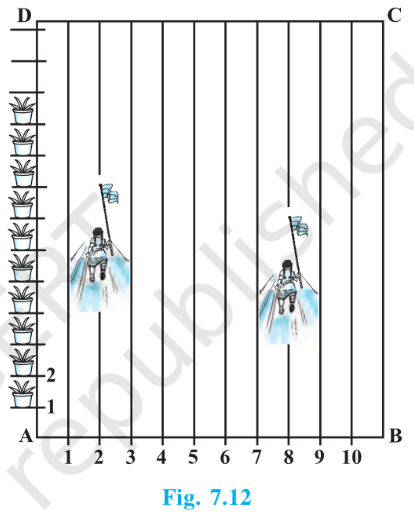
\includegraphics[width=\columnwidth]{./figs/sc.png}
  \caption{}
\label{fig:10/7/12Fig1}
\end{figure}               
      
\item Find the ratio in which the line segment joining the points $(-3,10) \text{ and } (6,-8)$ $\text{ is divided by } (-1,6)$.
\item Find the ratio in which the line segment joining $A(1,-5) \text{ and } B(-4,5)$ $\text{is divided by the x-axis}$. Also find the coordinates of the point of division.
\item If $(1,2), (4,y), (x,6), (3,5)$ are the vertices of a parallelogram taken in order, find x and y.
\item Find the coordinates of a point A, where AB is the diameter of a circle whose centre is $(2,-3) \text{ and }$ B is $(1,4)$.
\item If A \text{ and } B are $(-2,-2) \text{ and } (2,-4)$, respectively, find the coordinates of P such that AP= $\frac {3}{7}$AB $\text{ and }$ P lies on the line segment AB.
\item Find the coordinates of the points which divide the line segment joining $A(-2,2) \text{ and } B(2,8)$ into four equal parts.
\item Find the area of a rhombus if its vertices are $(3,0), (4,5), (-1,4) \text{ and } (-2,-1)$ taken in order. [$\vec{Hint}$ : Area of rhombus =$\frac {1}{2}$(product of its diagonals)]

\end{enumerate}

\end{document}